%%%%%%%%%%%%%%%%%%%%%%%%%%%%%%%%%%%%%%%%%%%%%%%%%%%%%%%%%%%%%%%%%%%%%%%%%%%%%%%%%
%%%%%%%%%%%%%%%%%%%%%%%%%%%%%%%%%%%%%%%%%%%%%%%%%%%%%%%%%%%%%%%%%%%%%%%%%%%%%%%%%
%%%%%%%%%%%%%%%%%%%%%%%%%%%%%%%%%%%%%%%%%%%%%%%%%%%%%%%%%%%%%%%%%%%%%%%%%%%%%%%%%
%%% slides stuff

\newcommand{\blocknode}[5]{\node (#1) at #2 {%
    \begin{minipage}{3.5cm}\begin{block}{#4}
        \begin{overlayarea}{3.5cm}{#3}
        #5\end{overlayarea}\end{block}\end{minipage}};}
\newcommand{\smallblocknode}[5]{\node (#1) at #2 {%
    \begin{minipage}{3.0cm}\begin{block}{#4} \begin{overlayarea}{3.0cm}{#3}
    #5\end{overlayarea}\end{block}\end{minipage}};}
\newcommand{\redsmallblocknode}[5]{\node (#1) at #2 {%
    \begin{minipage}{3.0cm}\begin{alertblock}{#4} \begin{overlayarea}{3.0cm}{#3}
    #5\end{overlayarea}\end{alertblock}\end{minipage}};}



\renewcommand{\newblock}{}
\definecolor{ToDoColor}{rgb}{0,0.16,0.90} %blue
\definecolor{OutlineColor}{rgb}{0.2,0.8,0.2} %green
\definecolor{CommentColor}{rgb}{0.90,0.16,0} %red
\definecolor{dkgreen}{rgb}{0,0.5,0}
\definecolor{mLightBrown}{rgb}{0.71,0.40,0.11}
\definecolor{mLightGreen}{rgb}{0.56,0.93,0.56}
\newcommand<>{\textblue}[1]{{\color#2{blue}#1}}
\newcommand<>{\textred}[1]{{\color#2{red}#1}}
\newcommand<>{\textgreen}[1]{{\color#2{green}#1}}
\newcommand<>{\textdkgreen}[1]{{\color#2{dkgreen}#1}}
\newcommand<>{\textorange}[1]{{\color#2{orange}#1}}
\newcommand<>{\textyellow}[1]{{\color#2{yellow}#1}}

\newcommand{\ie}{i.\,e.}
\newcommand{\eg}{e.\,g.}
\newcommand{\cf}{cf.}

\newcommand{\notesym}{\ensuremath{\to}} 
\newcommand{\noteblk}[1]{
\begin{block}{}
#1
\end{block}} 

\newcommand{\lectureslides}[1]{\ifthenelse{\value{VERSION}=0}{#1}{}}
\newcommand{\nolectureslides}[1]{\ifthenelse{\not\value{VERSION}=0}{#1}{}}
\newcommand{\posthandout}[1]{\ifthenelse{\value{VERSION}=1}{#1}{}}
\newcommand{\noposthandout}[1]{\ifthenelse{\not\value{VERSION}=1}{#1}{}}
\newcommand{\prehandout}[1]{\ifthenelse{\value{VERSION}=2}{#1}{}}
\newcommand{\noprehandout}[1]{\ifthenelse{\not\value{VERSION}=2}{#1}{}}


\newcommand{\images}{../IMAGES}
\graphicspath{{../IMAGES/}}
\newcommand{\rovergoal}[1]{
\includegraphics[scale=0.06]{rovergoal#1.png}
}


%%%%%%%%%%%%%%%%%%%%%%%%%%%%%%%%%%%%%%%%%%%
%%% defs, propositions, etc

\newenvironment{mydef}[1]{

\begin{block}{#1}
}{
\end{block}
}

\newenvironment{myprop}[1]{

\begin{block}{Proposition (#1)}
}{
\end{block}
}

\newenvironment{myproof}{

\begin{block}{Proof}
}{
\end{block}
}



%%%%%%%%%%%%%%%%%%%%%
%%%
%%% quiz: highlight ``correct'' (green, 2), ``discuss''
%%% (orange, 1), ``false'' (red, 0) in post-handouts only!

\newcommand{\quiz}[9]{

\prehandout{
\begin{block}{Quiz}
\textbf{#1}
\vspace{-0.15cm}
\begin{columns}
\begin{column}{.45\textwidth}
\begin{itemize}
\item[\textblue{(A):}] #2\vspace{-0.05cm}
\item[\textblue{(C):}] #4
\end{itemize}
\end{column}
\begin{column}{.45\textwidth}
\begin{itemize}
\item[\textblue{(B):}] #3\vspace{-0.05cm}
\item[\textblue{(D):}] #5
\end{itemize}
\end{column}
\end{columns}
\end{block}
}

\lectureslides{
\begin{block}{Quiz}
\textbf{#1}
\vspace{-0.15cm}
\begin{columns}
\begin{column}{.45\textwidth}
\begin{itemize}
\item[\textblue{(A):}] #2\vspace{-0.05cm}
\item[\textblue{(C):}] #4
\end{itemize}
\end{column}
\begin{column}{.45\textwidth}
\begin{itemize}
\item[\textblue{(B):}] #3\vspace{-0.05cm}
\item[\textblue{(D):}] #5
\end{itemize}
\end{column}
\end{columns}
\end{block}
}

\posthandout{
\begin{block}{Quiz}
\textbf{#1}
\vspace{-0.15cm}
\begin{columns}
\begin{column}{.45\textwidth}
\begin{itemize}
\item[\textblue{(A):}] \ifthenelse{#6=0}{\textred{#2}}{\ifthenelse{#6=1}{\textorange{#2}}{\ifthenelse{#6=2}{\textdkgreen{#2}}{}}}\vspace{-0.05cm}
\item[\textblue{(C):}] \ifthenelse{#8=0}{\textred{#4}}{\ifthenelse{#8=1}{\textorange{#4}}{\ifthenelse{#8=2}{\textdkgreen{#4}}{}}}
\end{itemize}
\end{column}
\begin{column}{.45\textwidth}
\begin{itemize}
\item[\textblue{(B):}] \ifthenelse{#7=0}{\textred{#3}}{\ifthenelse{#7=1}{\textorange{#3}}{\ifthenelse{#7=2}{\textdkgreen{#3}}{}}}\vspace{-0.05cm}
\item[\textblue{(D):}] \ifthenelse{#9=0}{\textred{#5}}{\ifthenelse{#9=1}{\textorange{#5}}{\ifthenelse{#9=2}{\textdkgreen{#5}}{}}}
\end{itemize}
\end{column}
\end{columns}
\end{block}
}

}




%%%%%%%%%%%%%%%%%%%%%
%%%
%%% quiztwo: highlight ``correct'' (green, 2), ``discuss''
%%% (orange, 1), ``false'' (red, 0) in post-handouts only!

\newcommand{\quiztwo}[5]{

\prehandout{
\begin{block}{Quiz}
\textbf{#1}
\vspace{-0.15cm}
\begin{columns}
\begin{column}{.45\textwidth}
\begin{itemize}
\item[\textblue{(A):}] #2
\end{itemize}
\end{column}
\begin{column}{.45\textwidth}
\begin{itemize}
\item[\textblue{(B):}] #3
\end{itemize}
\end{column}
\end{columns}
\end{block}
}

\lectureslides{
\begin{block}{Quiz}
\textbf{#1}
\vspace{-0.15cm}
\begin{columns}
\begin{column}{.45\textwidth}
\begin{itemize}
\item[\textblue{(A):}] #2
\end{itemize}
\end{column}
\begin{column}{.45\textwidth}
\begin{itemize}
\item[\textblue{(B):}] #3
\end{itemize}
\end{column}
\end{columns}
\end{block}
}

\posthandout{
\begin{block}{Quiz}
\textbf{#1}
\vspace{-0.15cm}
\begin{columns}
\begin{column}{.45\textwidth}
\begin{itemize}
\item[\textblue{(A):}] \ifthenelse{#4=0}{\textred{#2}}{\ifthenelse{#4=1}{\textorange{#2}}{\ifthenelse{#4=2}{\textdkgreen{#2}}{}}}
\end{itemize}
\end{column}
\begin{column}{.45\textwidth}
\begin{itemize}
\item[\textblue{(B):}] \ifthenelse{#5=0}{\textred{#3}}{\ifthenelse{#5=1}{\textorange{#3}}{\ifthenelse{#5=2}{\textdkgreen{#3}}{}}}
\end{itemize}
\end{column}
\end{columns}
\end{block}
}

}




%%%%%%%%%%%%%%%%%%%%%%%%%%%%%%%%%%%%%%%%%%%%%%%%%%%%%%%%%%%%%%%%%%%%%%%%%%%%%%%%%
%%%%%%%%%%%%%%%%%%%%%%%%%%%%%%%%%%%%%%%%%%%%%%%%%%%%%%%%%%%%%%%%%%%%%%%%%%%%%%%%%
%%%%%%%%%%%%%%%%%%%%%%%%%%%%%%%%%%%%%%%%%%%%%%%%%%%%%%%%%%%%%%%%%%%%%%%%%%%%%%%%%
%%% commands from paper

\newcommand{\defined}[1]{\textblue{#1}}


%%%%%%%%%%% heuristics %%%%%%%%%%%%

\newcommand{\hrefine}{\ensuremath{h_{r}}}
\newcommand{\hboth}{\ensuremath{h_{r+b}}}
\newcommand{\hbellman}{\ensuremath{h_{b}}}

\newcommand{\abs}{\mathcal{A}}
\newcommand{\numtasks}[1]{\tiny{(#1)}}

%\newcommand{\formalspacesave}{}

\newcommand{\naturals}{\ensuremath{\mathbb N}}
\newcommand{\reals}{{\mathbb{R}}}
\newcommand{\powerset}{{\mathcal{P}}}

\newcommand{\tuple}[1]{\ensuremath{\langle #1 \rangle}}

\newcommand{\astar}{\ensuremath{\textrm{A}^*}}

\newcommand{\poly}{\textbf{P}}
\newcommand{\np}{\textbf{NP}}
\newcommand{\pspace}{\textbf{PSPACE}}


%%%%%%%%%%%%%%%%%%%%%%%%%%%%%%
%%%%% Generic Framework
\newcommand{\task}{\ensuremath{\tau}}
%\newcommand{\task}{\ensuremath{\cal T}}
\newcommand{\plan}{\ensuremath{\pi}}
\newcommand{\plans}{\ensuremath{\Pi}}
%\newcommand{\alltasks}{\ensuremath{\cal T}}
\newcommand{\allplans}{\ensuremath{\cal P}}
\newcommand{\true}{\ensuremath{\mathit{true}}}
\newcommand{\false}{\ensuremath{\mathit{false}}}

\newcommand{\prop}{\ensuremath{p}}
\newcommand{\propq}{\ensuremath{q}}
\newcommand{\props}{\ensuremath{P}}
\newcommand{\propsatom}{\ensuremath{{P^{\text{\textup{A}}}}}}
\newcommand{\propscomp}{\ensuremath{{P^{\text{\textup{C}}}}}}

\newcommand{\modelsof}[2]{\ensuremath{{\cal M}_#1(#2)}}
\newcommand{\entails}[3]{\ensuremath{#1 \models #2 \Rightarrow #3}}
\newcommand{\notentails}[3]{\ensuremath{#1 \not\models #2 \Rightarrow #3}}
\renewcommand{\iff}[3]{\ensuremath{#1 \models #2 \Leftrightarrow #3}}
\renewcommand{\equiv}[2]{\ensuremath{[#2]_{#1}}}
%
%% \renewcommand{\implies}[1]{\ensuremath{\Rightarrow_{#1}}}
%% \renewcommand{\iff}[1]{\ensuremath{\Leftrightarrow_{#1}}}
%% \renewcommand{\equiv}[2]{\ensuremath{[#1]_{#2}}}

\newcommand{\pdo}[1]{\ensuremath{\Rightarrow_{#1}}}
\newcommand{\pda}[1]{\ensuremath{\Phi_{#1}}}

\newcommand{\entailsuff}{\ensuremath{\Rightarrow_{\mathit{suff}}}}

\newcommand{\deps}{\ensuremath{D}}


%%%%%%%%%%%%%%%%%%%%%%%%%%%%%%
%%%%% Planning Tasks

\newcommand{\vars}{\ensuremath{V}}
\newcommand{\acts}{\ensuremath{A}}
\newcommand{\init}{\ensuremath{I}}
\newcommand{\goal}{\ensuremath{G}}
\newcommand{\goalhard}{\ensuremath{G^{\text{\textup{hard}}}}}
\newcommand{\goalsoft}{\ensuremath{G^{\text{\textup{soft}}}}}
\newcommand{\cost}{{\ensuremath{c}}}
\newcommand{\pre}{\ensuremath{\mathit{pre}}}
\newcommand{\eff}{\ensuremath{\mathit{eff}}}

\newcommand{\variables}[1]{\ensuremath{{\cal V}(#1)}}
\newcommand{\apply}[1]{\ensuremath{[[#1]]}}

\newcommand{\costbound}{{\ensuremath{b}}}


%%%%%%%%%%%%%%%%%%%%%%%%%%%%%%
%%%%% Goal facts

\newcommand{\goalpropsatom}{\ensuremath{{P^{\text{\textup{GA}}}}}}
\newcommand{\goalpropscomp}{\ensuremath{{P^{\text{\textup{GC}}}}}}

\newcommand{\geprops}{\ensuremath{{P^{\text{\textup{GE}}}}}}
\newcommand{\gedeps}{\ensuremath{{D^{\text{\textup{GE}}}}}}

\newcommand{\dgeprops}{\ensuremath{{P^{\text{\textup{DGE}}}}}}
\newcommand{\dgedeps}{\ensuremath{{D^{\text{\textup{DGE}}}}}}



%%%%%%%%%%%%%%%%%%%%%%%%%%%%%%
%%%%% Heuristic Functions

\newcommand{\hstar}{\ensuremath{h^*}}
\newcommand{\hplus}{\ensuremath{h^+}}

\newcommand{\hone}{\ensuremath{h^1}}
\newcommand{\htwo}{\ensuremath{h^2}}
\newcommand{\hm}{\ensuremath{h^m}}
\newcommand{\hc}{\ensuremath{h^C}}
\newcommand{\hcx}{\ensuremath{h^{C \cup X}}}
\newcommand{\uc}{\ensuremath{u^C}}
\newcommand{\ucx}{\ensuremath{u^{C \cup X}}}
\newcommand{\hmax}{\ensuremath{h^{\text{\textup{max}}}}}
\newcommand{\hff}{\ensuremath{h^{\text{\textup{FF}}}}}
\newcommand{\hlmcut}{\ensuremath{h^{\text{\textup{LM-cut}}}}}
\newcommand{\hms}{\ensuremath{h^{\text{M\&S}}}}


%%%%%%%%%%%%%%%%%%%%%%%%%%%%%%
%%%%% Stackelberg notation

\newcommand{\leader}{\ensuremath{L}}
\newcommand{\follower}{\ensuremath{F}}

\newcommand{\bestresponse}{\ensuremath{{BR}}}

\newcommand{\actsL}{\ensuremath{\acts^{\leader}}}
\newcommand{\actsF}{\ensuremath{\acts^{\follower}}}
\newcommand{\goalF}{\goal^{\follower}}

\newcommand{\statesL}{\ensuremath{\states^{\leader}}}

\newcommand{\equilibrium}{\ensuremath{\states^*}}

\newcommand{\strategyL}{\ensuremath{\strategy^{\leader}}}
\newcommand{\strategyF}{\ensuremath{\strategy^{\follower}}}

\newcommand{\strategystarL}{\ensuremath{\strategy^{\leader*}}}
\newcommand{\strategystarF}{\ensuremath{\strategy^{\follower*}}}

\newcommand{\costL}{\ensuremath{\leader}}
\newcommand{\costF}{\ensuremath{\follower}}
\newcommand{\coststarL}{\ensuremath{\leader^*}}
\newcommand{\coststarF}{\ensuremath{\follower^*}}
\newcommand{\costapproxL}{\ensuremath{\leader^+}}
\newcommand{\costapproxF}{\ensuremath{\follower^+}}

\newcommand{\hstackel}{\ensuremath{h^{\text{\textup{Stackel}}}}}
\newcommand{\Hstackel}{\ensuremath{H}}
\newcommand{\upperF}{\ensuremath{\mathsf{up}^{\follower}}}
\newcommand{\lowerL}{\ensuremath{\mathsf{low}^{\leader}}}
\newcommand{\upperL}{\ensuremath{\mathsf{up}^{\leader}}}

%%%%%%%%%%%%%%%%%%%%%%%%%%%%%%
%%%%% Search algorithms

\newcommand{\result}{\ensuremath{\hat{S}}}

\newcommand{\open}{\ensuremath{\mathsf{Open}}}
\newcommand{\closed}{\ensuremath{\mathsf{Explored}}}
\newcommand{\comment}[1]{{\color{red} /* #1 */}}

\newcommand{\searchalg}{\ensuremath{\textup{leader-follower-search}}}

\newcommand{\bounds}{\ensuremath{\mathbb{B}}}

%%% Planning domains
\newcommand{\airport}               {{Airport}}
\newcommand{\barman }               {{Barman}}
\newcommand{\blocksworld}           {{Blocksworld}}
\newcommand{\childsnack}           {{Childsnack}}
\newcommand{\depots}                {{Depots}}
\newcommand{\driverlog}             {{Driverlog}}
\newcommand{\elevators}             {{Elevators}}
\newcommand{\floortile}             {{Floortile}}
\newcommand{\freecell}              {{FreeCell}}
\newcommand{\grid}                  {{Grid}}
\newcommand{\gripper}               {{Gripper}}
\newcommand{\hiking}               {{Hiking}}
\newcommand{\logistics}             {{Logistics}}
\newcommand{\simplelogistics}       {{Simple-Logistics}}
\newcommand{\movie}                 {{Movie}}
\newcommand{\extmovie}              {{Ext-Movie}}
\newcommand{\promela}               {{Promela}}
\newcommand{\diningphilosophers}    {{Dining-Philosophers}}
\newcommand{\opticaltelegraph}      {{Optical-Telegraph}}
\newcommand{\miconic}               {{Miconic}}
\newcommand{\mystery}               {{Mystery}}
\newcommand{\mprime}                {{Mprime}}
\newcommand{\nomystery}             {{Nomystery}}
\newcommand{\openstacks}            {{Openstacks}}
\newcommand{\parcprinter}           {{Parcprinter}}
\newcommand{\parking}               {{Parking}}
\newcommand{\pathways}              {{Pathways}}
\newcommand{\pegsol}                {{Pegsol}}
\newcommand{\pipesworld}            {{Pipesworld}}
\newcommand{\pipesworldnotankage}   {{Pipesworld-NoTankage}}
\newcommand{\pipesworldtankage}     {{Pipesworld-Tankage}}
\newcommand{\pipesworldnotankageshort}   {{Pipes-NoTank}}
\newcommand{\pipesworldtankageshort}     {{Pipes-Tank}}
\newcommand{\psr}                   {{PSR}}
\newcommand{\rovers}                {{Rovers}}
\newcommand{\satellite}             {{Satellite}}
\newcommand{\scanalyzer}            {{Scanalyzer}}
\newcommand{\schedule}              {{Schedule}}
\newcommand{\schedulestrips}        {{Schedule-Strips}}
\newcommand{\seqschedule}           {{SeqSchedule}}
\newcommand{\sokoban}               {{Sokoban}}
\newcommand{\storage}               {{Storage}}
\newcommand{\tetris}               {{Tetris}}
\newcommand{\thoughtful}               {{Thoughtful}}
\newcommand{\tidybot}               {{Tidybot}}
\newcommand{\tpp}                   {{TPP}}
\newcommand{\trucks}                {{Trucks}}
\newcommand{\transport}             {{Transport}}
\newcommand{\woodworking}           {{Woodworking}}
\newcommand{\woodworkingshort}      {{Woodwork}}
\newcommand{\visitall}              {{Visitall}}
\newcommand{\zenotravel}            {{Zenotravel}}

\newcommand{\airportveryshort}{Airport}
\newcommand{\barmanveryshort}{Barman}
\newcommand{\blocksworldveryshort}{Blocksworld}
\newcommand{\childsnackveryshort}           {{Childsnack}}
\newcommand{\depotsveryshort}{Depots}
\newcommand{\driverlogveryshort}{Driverlog}
\newcommand{\elevatorsveryshort}{Elevators}
\newcommand{\floortileveryshort}{Floortile}
\newcommand{\freecellveryshort}{Freecell}
\newcommand{\gripperveryshort}{Gripper}
\newcommand{\gridveryshort}{Grid}
\newcommand{\hikingveryshort}               {{Hiking}}
\newcommand{\logisticsveryshort}{Logistics}
\newcommand{\miconicveryshort}{Miconic}
\newcommand{\mprimeveryshort}{Mprime}
\newcommand{\mysteryveryshort}{Mystery}
\newcommand{\nomysteryveryshort}{NoMystery}
\newcommand{\openstacksveryshort}{Openstacks}
\newcommand{\parkingveryshort}{Parking}
\newcommand{\parcprinterveryshort}{Parcprinter}
\newcommand{\pathwaysveryshort}{Pathways}
\newcommand{\pegsolveryshort}{Pegsol}
\newcommand{\pipesworldnotankageveryshort}   {{PipesNoTank}}
\newcommand{\pipesworldtankageveryshort}     {{PipesTank}}
\newcommand{\psrveryshort}{PSR}
\newcommand{\roversveryshort}{Rovers}
\newcommand{\satelliteveryshort}{Satellite}
\newcommand{\scanalyzerveryshort}{Scanalyzer}
\newcommand{\sokobanveryshort}{Sokoban}
\newcommand{\storageveryshort}               {{Storage}}
\newcommand{\tetrisveryshort}               {{Tetris}}
\newcommand{\thoughtfulveryshort}       {{Thoughtful}}
\newcommand{\tidybotveryshort}{Tidybot}
\newcommand{\tppveryshort}{TPP}
\newcommand{\transportveryshort}{Transport}
\newcommand{\trucksveryshort}{Trucks}
\newcommand{\visitallveryshort}{Visitall}
\newcommand{\woodworkingveryshort}{Woodworking}
\newcommand{\zenotravelveryshort}{Zenotravel}

\newcommand{\pentesting}{{Pentest}}
\newcommand{\pentestingshort}{{Pentest}}





%%%%%%%%%%%%%%%%%%%%%%%%%%%%%%%%%%%%%%%%%%%%%%%%%%%%%%%%%%%%%%%%%%%%%%%%%%%%%%%%%
%%%%%%%%%%%%%%%%%%%%%%%%%%%%%%%%%%%%%%%%%%%%%%%%%%%%%%%%%%%%%%%%%%%%%%%%%%%%%%%%%
%%%%%%%%%%%%%%%%%%%%%%%%%%%%%%%%%%%%%%%%%%%%%%%%%%%%%%%%%%%%%%%%%%%%%%%%%%%%%%%%%
%%% commands for Rebecca's illustrations

\newcommand{\samerover}[2]{
	\begin{tikzpicture}
		\node[] (r1) at (-0.7,0) {
\includegraphics[scale=0.04]{rover1.png}};
		\node[] (xor) at (0.05,0) {$\otimes$};
		\node[] (r2) at (0.7,0) {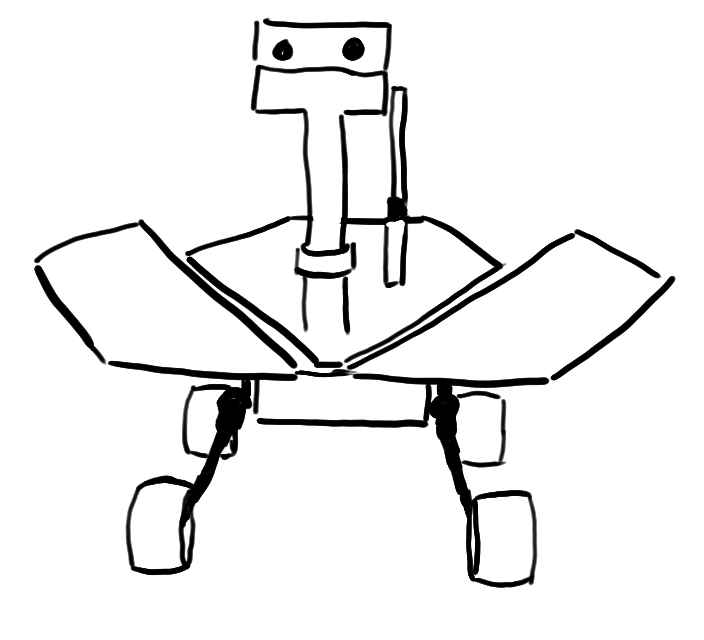
\includegraphics[scale=0.04]{rover2.png}};
		\node[] (i1) at (-0.5,1) {\includegraphics[scale=0.06]{rovergoal#1.png}};
		\node[] (i2) at (0.5,1) {\includegraphics[scale=0.06]{rovergoal#2.png}};
		\node[] (n) at (0,-0.7) {same rover};
	\end{tikzpicture}
}


\newcommand{\energylimit}[1]{
	\begin{tikzpicture}
		\node[] (i1) at (0,1) {\includegraphics[scale=0.06]{rovergoal#1.png}};
		\node[] (i2) at (-0.5,0) {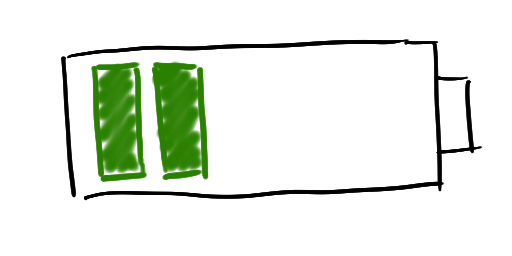
\includegraphics[scale=0.06]{battery-low.png}};
		\node[] (p) at (0.8,0) {\large $> 50\%$};
		\node[] (n) at (0,-0.7) {energy limit};
	\end{tikzpicture}
}

\newcommand{\orderprop}[2]{
	\begin{tikzpicture}
		\node[] (i11) at (-0.5,1.2) {$1.$};
		\node[] (i1) at (-0.5,0.5) {\includegraphics[scale=0.06]{rovergoal#1.png}};
		\node[] (i11) at (0.5,1.2) {$2.$};
		\node[] (i2) at (0.5,0.5) {\includegraphics[scale=0.06]{rovergoal#2.png}};
		\node[] (n) at (0,-0.7) {order};
	\end{tikzpicture}
}


\newcommand{\specificrover}[2]{
	\begin{tikzpicture}
		\node[] (r1) at (0,0) {\includegraphics[scale=0.05]{rover#1.png}};
		\node[] (i2) at (0,1) {\includegraphics[scale=0.06]{rovergoal#2.png}};
		\node[] (n) at (0,-0.7) {specific rover};
	\end{tikzpicture}
}


\newcommand{\useconnection}[3]{
	\begin{tikzpicture}
		\node[] (r1) at (0,0.3) {\includegraphics[scale=0.05]{rover#1.png}};
		\node[draw, circle, inner sep=1pt] (Lx) at (-1,-0.5) {\small $L_#2$};
		\node[draw, circle, inner sep=1pt] (Ly) at (1,-0.5) {\small $L_#3$};
		\draw[thick, <->] (Lx) to (Ly);
		\node[] (n) at (0,-1) {use connection};
	\end{tikzpicture}
}


\newcommand{\dontuseconnection}[3]{
	\begin{tikzpicture}
		\node[] (r1) at (0,0.3) {\includegraphics[scale=0.05]{rover#1.png}};
		\node[] (r1) at (0,-0.45) {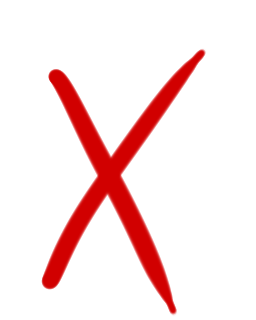
\includegraphics[scale=0.08]{no.png}};
		\node[draw, circle, inner sep=1pt] (Lx) at (-1,-0.5) {\small $L_#2$};
		\node[draw, circle, inner sep=1pt] (Ly) at (1,-0.5) {\small $L_#3$};
		\draw[thick, <->] (Lx) to (Ly);
		\node[align=center] (n) at (0,-1.1) {don't use\\[-0.3cm]connection};
	\end{tikzpicture}
}


\newcommand{\energylimitloc}[1]{
	\begin{tikzpicture}
		\node[] (r1) at (0,0) {\includegraphics[scale=0.05]{rover#1.png}};
		\node[] (b1) at (-0.5,1) {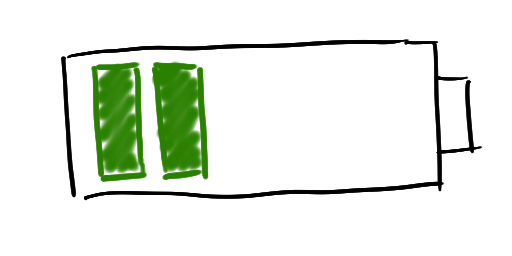
\includegraphics[scale=0.06]{battery-low.png}};
		\node[draw, circle, inner sep=1pt] (l) at (0.5,1) {$L_y$};
		\node[] (n) at (0,-0.7) {energy limit};
	\end{tikzpicture}
}













